
%%%%%%%%%%%%%%%%%%%%%%%%%%%%%%%%%%%%%%%%%%%%%%%%%%%%%%%%%%%%%%%%%%%%%
%% This is a (brief) model paper using the achemso class
%% The document class accepts keyval options, which should include
%% the target journal and optionally the manuscript type.
%%%%%%%%%%%%%%%%%%%%%%%%%%%%%%%%%%%%%%%%%%%%%%%%%%%%%%%%%%%%%%%%%%%%%
\documentclass[journal=jctcce,manuscript=article]{achemso}
\setkeys{acs}{articletitle=true}
%%%%%%%%%%%%%%%%%%%%%%%%%%%%%%%%%%%%%%%%%%%%%%%%%%%%%%%%%%%%%%%%%%%%%
%% Place any additional packages needed here.  Only include packages
%% which are essential, to avoid problems later.
%%%%%%%%%%%%%%%%%%%%%%%%%%%%%%%%%%%%%%%%%%%%%%%%%%%%%%%%%%%%%%%%%%%%%
\usepackage{chemformula} % Formula subscripts using \ch{}
\usepackage[T1]{fontenc} % Use modern font encodings
\usepackage{lmodern}
\usepackage{amsmath,amssymb}
\usepackage{graphicx}
\usepackage{float}
\usepackage{braket}
\usepackage{multirow}
\usepackage{array}
\usepackage{lipsum}
\usepackage[normalem]{ulem}
\usepackage[xcolor,leftbars]{changebar}
\newcolumntype{R}{>{$}r<{$}}
\newcolumntype{C}{>{$}c<{$}}
%%%%%%%%%%%%%%%%%%%%%%%%%%%%%%%%%%%%%%%%%%%%%%%%%%%%%%%%%%%%%%%%%%%%%
%% If issues arise when submitting your manuscript, you may want to
%% un-comment the next line.  This provides information on the
%% version of every file you have used.
%%%%%%%%%%%%%%%%%%%%%%%%%%%%%%%%%%%%%%%%%%%%%%%%%%%%%%%%%%%%%%%%%%%%%
%%\listfiles

%%%%%%%%%%%%%%%%%%%%%%%%%%%%%%%%%%%%%%%%%%%%%%%%%%%%%%%%%%%%%%%%%%%%%
%% Place any additional macros here.  Please use \newcommand* where
%% possible, and avoid layout-changing macros (which are not used
%% when typesetting).
%%%%%%%%%%%%%%%%%%%%%%%%%%%%%%%%%%%%%%%%%%%%%%%%%%%%%%%%%%%%%%%%%%%%%
%\newcommand{\reviewer}[1]{\vspace{0.5cm}\noindent\textbf{#1}}
\newcommand{\response}[1]{\vspace{0.25cm} \textit{#1}}
\newcommand{\excerpt}[1]{\vspace{0.25cm} {#1}}
\newcommand*{\rev}[1]{{\color{blue} #1}}
\newcommand{\filipp}[1]{{\color{red} #1}}
\cbcolor{red}
\newenvironment{reviewer}%
{\begin{quote}%
  \begin{changebar}\cbcolor{gray}\color{black}}%
  {\end{changebar}%
\end{quote}}
%%%%%%%%%%%%%%%%%%%%%%%%%%%%%%%%%%%%%%%%%%%%%%%%%%%%%%%%%%%%%%%%%%%%%
%% Meta-data block
%% ---------------
%% Each author should be given as a separate \author command.
%%
%% Corresponding authors should have an e-mail given after the author
%% name as an \email command. Phone and fax numbers can be given
%% using \phone and \fax, respectively; this information is optional.
%%
%% The affiliation of authors is given after the authors; each
%% \affiliation command applies to all preceding authors not already
%% assigned an affiliation.
%%
%% The affiliation takes an option argument for the short name.  This
%% will typically be something like "University of Somewhere".
%%
%% The \altaffiliation macro should be used for new address, etc.
%% On the other hand, \alsoaffiliation is used on a per author basis
%% when authors are associated with multiple institutions.
%%%%%%%%%%%%%%%%%%%%%%%%%%%%%%%%%%%%%%%%%%%%%%%%%%%%%%%%%%%%%%%%%%%%%
\author{Brian D. Nguyen}
\author{Guo P. Chen}
\author{Matthew M. Agee}
\author{Asbj{\"o}rn M. Burow}
\author{Matthew P. Tang}
\author{Filipp Furche}
\affiliation{Department of Chemistry, University of California, Irvine,
    1102 Natural Sciences II, Irvine, CA 92697-2025, USA}
\email{filipp.furche@uci.edu}
%%%%%%%%%%%%%%%%%%%%%%%%%%%%%%%%%%%%%%%%%%%%%%%%%%%%%%%%%%%%%%%%%%%%%
%% The document title should be given as usual. Some journals require
%% a running title from the author: this should be supplied as an
%% optional argument to \title.
%%%%%%%%%%%%%%%%%%%%%%%%%%%%%%%%%%%%%%%%%%%%%%%%%%%%%%%%%%%%%%%%%%%%%
\title[Review]{Responses to Reviewers' comments for
  Divergence of Many-Body Perturbation Theory for Noncovalent
  Interactions of Large Molecules}

%%%%%%%%%%%%%%%%%%%%%%%%%%%%%%%%%%%%%%%%%%%%%%%%%%%%%%%%%%%%%%%%%%%%%
%% The manuscript does not need to include \maketitle, which is
%% executed automatically.
%%%%%%%%%%%%%%%%%%%%%%%%%%%%%%%%%%%%%%%%%%%%%%%%%%%%%%%%%%%%%%%%%%%%%
\begin{document}

%%%%%%%%%%%%%%%%%%%%%%%%%%%%%%%%%%%%%%%%%%%%%%%%%%%%%%%%%%%%%%%%%%%%%
%% Start the main part of the manuscript here.
%%%%%%%%%%%%%%%%%%%%%%%%%%%%%%%%%%%%%%%%%%%%%%%%%%%%%%%%%%%%%%%%%%%%%


\clearpage

%\filipp{Spell-check the whole thing (but not the reviewers comments,
%  they need to be verbatim)}

We apologize for the delay and thank the Reviewers for taking the time
to read the manuscript, and for their helpful and constructive comments. 

Changes made to the manuscript are displayed in blue; in addition, a
version of the manuscript showing all changes made is provided. 

\section*{Reviewer 1}

\begin{reviewer}
  This is a really interesting paper that investigates the performance of
  Moller-Plesset perturbation theory (especially MP2) and the random phase
  approximation for the treatment of non-covalent interactions. The paper
  stands out for its development of a new flavor of perturbation theory
  that can be reduced to either RPA or many-body perturbation theory (MBPT)
  models. The authors use this approach to show divergence and breakdown
  of MBPT in large systems.  The work is well done, with both formal
  theoretical developments and numerical evidence to support their arguments.
  I expect it will spur interesting discussions in the field. I definitely
  recommend publication after modest revisions described below.
\end{reviewer}
  
\begin{reviewer}
  1) The choice of reference values used in the L7 and S30L benchmark systems
  is a potential issue.  The authors, like many others, are using reference
  data computed with DLPNO-CCSD(T) by computational necessity.  However, the
  user-chosen parameters in DLPNO can dramatically impact the benchmark values
  obtained. For example, the L7 data set reference values from Ref 78 and
  some summarized in Table 4 of 10.1021/acs.jpclett.9b01156 span many kcal/mol
  in some cases!
  
  The specific choice of reference data won't alter the essential story here
  that MP2 performs very poorly in these large systems, but it does potentially
  impact the performance assessment of the other models that do not exhibit such
  catastrophic behavior.  I don't have a strong opinion about which of the L7
  and S30L reference values they should use, but I do think they should be more
  explicit about the uncertainty surrounding the ``true'' values and why they
  chose the reference data they did.
\end{reviewer}

We agree with the Reviewer that the choice of thresholds that control
truncation of the PNO basis and domain size can significantly affect
binding energies. The DLPNO-CCSD(T) references chosen for this study
used the ``tightPNO'' parameters from Refs \citenum{doi:10.1021/acs.jpclett.9b01156}
and \citenum{doi:10.1021/ct501129s}. In response to the Reviewer's
comment, the manuscript was revised as follows:

``The interaction energies were benchmarked against CCSD(T)
  values for the S66 benchmark \rev{set\cite{doi:10.1021/ct2002946,doi:10.1021/ct200523a}}
  and against the \rev{domain-based local pair-natural orbital (DLPNO)
    based CCSD(T) calculations for the L7 and S30L benchmark
  sets.\cite{doi:10.1063/1.5090222,doi:10.1063/1.5012601}}
  \rev{DLPNO-CCSD(T) results can vary significantly for weakly bound
    complexes depending on the truncation of the PNO basis and domain
    size.\cite{doi:10.1021/ct501129s,doi:10.1021/acs.jpclett.9b01156}
    Moreover, even with tight truncation thresholds, the results may
    differ by up to $\sim$2 kcal/mol based on the choice of basis set
    and basis-set extrapolation scheme as seen between
    Refs.~\citenum{doi:10.1063/1.5012601} and
    \citenum{doi:10.1021/acs.jpclett.9b01156}. For the
      present study, 
    the DLPNO-CCSD(T) reference values were taken from Brandenburg
    \textit{et al}\cite{doi:10.1063/1.5012601} employing the ``TightPNO''
    truncations with the basis-set extrapolation scheme from
    Ref. \citenum{doi:10.1021/acs.jctc.5b00515}
    for both the L7 and S30L benchmarks.} Throughout \rev{the} paper,
    signed errors are defined as differences between calculated and
    reference values; for example, a positive error in binding energies
    signifies underbinding.'' (p. 7)

\begin{reviewer}
2) I would like the authors to elaborate on the connection between the
breakdown of MP2 identified here and the older intermolecular perturbation
theory literature on the problems of the uncoupled Hartree-Fock.  At present,
it's unclear to me whether the authors' new approach is ``just'' a different
way of framing the older UCHF dispersion issues combined with nice numerical
evidence that the problem becomes catastrophic in large systems, or if there
is something going on beyond that problem.

For example, MP2C uses those older ideas to replace the UCHF dispersion with
a better coupled Kohn-Sham treatment that isn't all that different to RPA.
MP2C certainly cleans up the MP2 issues in S66 and L7: Using the L7 data on
BEGDB.com and the reference data from Ref 78, I compute, in kcal/mol:
\end{reviewer}

\begin{table}
  \begin{tabular}{c|ccc}
    & ME &   MAE &  MinMax \\
    \hline
    MP2   &  -8.1  &  8.1 &  17.5 \\
    MP2C  &  -0.2  &  0.5 &  2.4 \\
    MP2.5 &  -0.9  &  1.1 &  2.0
  \end{tabular}
\end{table}
\begin{reviewer}
These are clearly on par with the best DFT models you show and out-performing RPA.
For S66, the ME, MAE, and MinMax of MP2C are something like -0.0, 0.1, and 0.5
kcal/mol, which are considerably smaller than any of the other methods shown in
Table 1.

Given this, I would be curious to know, for example, what Fig 9/Table 2 look
like for MP2C.  Would we still see considerable divergence in the largest systems?
Or is the MP2C just slowing down the divergence onset, but not curing it? Perhaps
a different way of addressing this: Can it be determined from the present perturbation
theory approach if subtracting out the uncoupled Hartree-Fock dispersion in MP2
(as is done in MP2C) removes the divergence?
\end{reviewer}

We thank the Reviewer for the comment. We added Sec. 4.5.3 to the
manuscript to address this question in detail. It turns out that
``just'' addressing the issues of UCHF is not sufficient for large and
polarizable monomers. 

\noindent\rev{\textbf{4.5.3 MP2C: Partial Resummation of MBPT}}

\rev{He{\ss}elmann's MP2C method \cite{doi:10.1063/1.2905808,
    Pitonak10JChemTheoryComput6p168,doi:10.1063/1.4809981}
  replaces
the (uncoupled) LHZK(2) part of the MP2 interaction energy with its
(coupled) time-dependent DFT counterpart. In the large-$R$ asymptotic
limit, time-dependent DFT reduces to RPA, and hence MP2C corresponds
to the replacements
\begin{equation}
  \label{eq:pt2cep}
\mathbf{K}^{\alpha\text{HXC}}_\text{int}(z)
\rightarrow \alpha \mathbf{V}_{\text{int}}\quad \text{and} \quad
\boldsymbol{\Pi}^0(z) 
\rightarrow \boldsymbol{\Pi}^{\text{RPA}}(z) \quad \text{and} \quad
\boldsymbol{\kappa}_{\alpha}(z) \rightarrow \mathbf{1}
\end{equation}
in Eqs. (13)-(23). Equivalently, MP2C may be
understood as a low-order approximation to the RPA dispersion energy
resulting from first-order truncation of the Taylor expansion of $\ln
\boldsymbol{\kappa}^{\text{RPA}}(z)$ in Eq. (34) around
$\boldsymbol{\kappa}^{\text{RPA}}(z) = \mathbf{1}$,
\begin{equation}
  \label{eq:ecabmp2c}
  E^{\text{C\, PT2C}}_{\text{int}}[\rho] = \frac{1}{4}
  \int_{-\infty}^{\infty} \frac{d\omega}{2\pi} \langle 
    \boldsymbol{\kappa}^{\text{RPA}}(z) - \mathbf{1} \rangle.
\end{equation}
In other words, MP2C includes intramonomer screening effects to infinite
order, but the intermonomer interaction is second order only. The
convergence of this partially resummed MBPT series is more benign
compared to standard MBPT, because, for non-degenerate monomers, the
eigenvalues of $\boldsymbol{\kappa}^{\text{RPA}}(z)$ are between 0 and
1, and hence the Taylor expansion of  $\ln
\boldsymbol{\kappa}^{\text{RPA}}(z)$ converges. Also,
since $\ln x \leq x-1$ for $0 <x \leq 1$, the MP2C dispersion energy is
an upper bound for the RPA dispersion energy. However, 
with decreasing eigenvalues of $\boldsymbol{\kappa}^{\text{RPA}}(z)$,
i.e., for large and polarizable monomers, this Taylor series converges
increasingly slowly (and eventually diverges under DG conditions), and hence
this bound deteriorates rapidly. This is consistent with the observation
that MP2C underestimates binding energies of larger complexes contained
in the L7 benchmark \cite{doi:10.1021/ct400036b}.
Unlike the previously discussed RPA and MBPT approximations,
the MP2C method does not possess a ``seamless'' supermolecular
equivalent, i.e., it requires an SAPT-style partitioning 
into monomers, because the inter- and intramonomer interactions are
treated at different levels. From a computational viewpoint, truncation
of the Taylor expansion of $\ln \boldsymbol{\kappa}^{\text{RPA}}(z)$ offers
little advantage compared to full RPA using Eq. (34).}

\rev{Fig. \ref{fig:mp2c_rpa} summarizes the approximations to the AC-SAPT
dispersion energy discussed in this section in diagrammatic form.}
\begin{figure}[H]
  \centering
  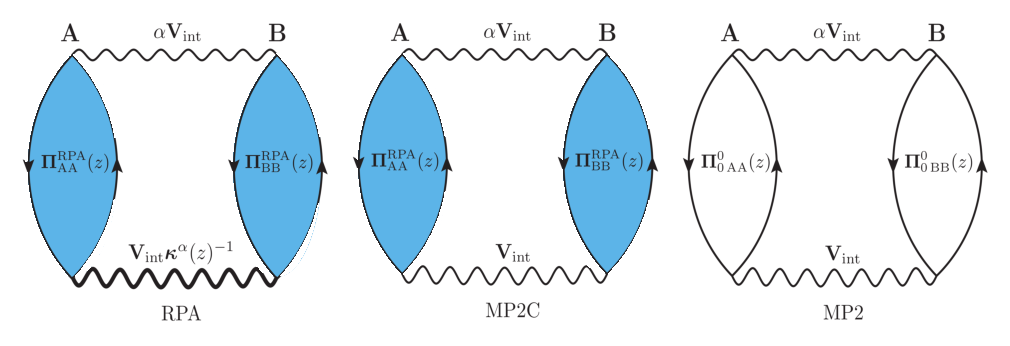
\includegraphics{int_gold_combine.eps}
  \caption{\rev{Diagrammatic representations of the A--B dispersion energy
    within RPA, MP2C, and MP2. Blue-shaded and empty rings
    with upward--downward arrows denote particle--hole propagators
    of the monomers containing the full and zero intra-monomer
    interaction, respectively,
    whereas horizontal wavy lines represent interactions between the
    monomers. Coupling strength and frequency integration are
    implied.}}
  \label{fig:mp2c_rpa}
\end{figure}

\begin{reviewer}
Overall, the authors' prognosis that MBPT should not be used for non-covalent
interactions in large systems seems overly grim, unless they show evidence
that these more robust models like MP2C that people currently use instead of
MP2 fail similarly.

[ Just to be clear, MP2C definitely has its own flaws: for example, it's purely
intermolecular, and in only corrects the interactions between pairs of molecules
(not trimers, etc). There have been efforts to address those weaknesses, such
as adding Axilrod-Teller terms to MP2, and/or MP2D, a variant of MP2C that does
handle both intra- and intermolecular interactions, but each of those also has
limitations.]

\end{reviewer}

We respectfully disagree with the reviewer on this point. Our analysis
provides substantial evidence, both theoretical and numerical, to
support the conclusion that conventional MBPT diverges in the vast
majority of applications, and must be expected to fail catastrophically
for large and polarizable systems. It is our goal to
communicate this point clearly and crisply to the community of users and
developers of electronic structure methods, without unduly over- or
understating it.

MP2C shares some characteristics with bare MBPT and some with RPA, but
it is not the main object of this paper nor particularly widely used
compared to supermolecular MBPT calculations. Nevertheless, in the
interest of a balanced presentation, we have
added the following paragraph to the conclusions:

\rev{``The MP2C method can be viewed as a partial MBPT resummation which
  includes intramonomer screening and exhibits better analytical properties
  than bare MPBT, but truncates intermonomer interactions at second order,
  and has no obvious supermolecular equivalent. For increasingly large
  and polarizable monomers, MP2C underestimates the magnitude of
  dispersion interactions progressively due to missing many-body
  dispersion.''} (p. 34)


\begin{reviewer}
3) Contrary to pg 4, line 51, I would not call MP2C empirical.  There is some
arbitrariness in the choice of functional for the CKS part, but the basic approach
doesn't contain fitted parameters of the sort usually associated with empirical
corrections.
\end{reviewer}

Although we feel that there is an element of empiricism in a method that
combines different references for computing different parts of the
energy, we have modified the sentence on p. 4 as suggested:

``For large molecular complexes, the shortcomings of pairwise additive methods
  such as MP2 have been ascribed to missing three- and higher-body dispersion
  interactions,\cite{Grimme12ChemEurJ18p9955} triggering the development of
  \rev{dispersion} corrections
  including MP2C,\cite{doi:10.1063/1.2905808,Pitonak10JChemTheoryComput6p168,
    doi:10.1063/1.4809981}
  \rev{MP2D,\cite{doi:10.1021/acs.jctc.8b00548,C9SC05689K}} as
  well as empirical three-\cite{Grimme12ChemEurJ18p9955,
    Caldeweyher17JChemPhys147p034112},
  and many-body\cite{Tkatchenko12PhysRevLett108p236402} \rev{\sout{empirical}}
  dispersion corrections for DFAs.'' (p. 4)

\begin{reviewer}
4) The Methods section lacks some details:
- How are the MP2 calculations performed?  Basis sets, etc. Are they in the
same def2-xZVP basis sets, without diffuse functions?
\end{reviewer}

The MP2 calculations used the same basis set methodology as the RPA
ones. Diffuse augmentation was not used since it produces linear dependencies
for the total energies of large systems in L7 and S30L. The basis set
convergence studies in Ref. \citenum{Eshuis12JChemPhys136p084105}
and reported in the appendix suggest that residual basis set
error is less than 1-2 kcal/mol, estimated conservatively.

To clarify this point, we added on p. 8: 

\rev{``Similarly, correlation energies from MP2 and its variants
    were obtainedusing the frozen core approximation, $50\%$ CP correction,
    and the 3-4 extrapolation using cc-pVTZ and cc-pVQZ basis
    sets\cite{Dunning89JChemPhys90p1007,doi:10.1063/1.464303}.
    HF energies were computed using def2-QZVP basis
    set\cite{Weigend05PhysChemChemPhys7p3297,Weigend03JChemPhys119p12753}.''}
(p. 8)
    
\begin{reviewer}
  Do the D3 corrections include the Axilrod-Teller-Muto terms?  Those are
  sometimes argued to be important in large systems.
\end{reviewer}

The semilocal density functional approximations with D3 corrections do
indeed include the Axilrod-Teller-Muto terms, see Ref.
\citenum{Sure15JChemTheoryComput}.

\begin{reviewer}
5) (optional) I was not familiar with the ``per mille'' variant of the
percentage sign.  That might just reflect my own ignorance, but it might
help to either define it or switch units to percentages to reduce confusion.
\end{reviewer}

The ``per mille'' (\textperthousand) sign was replaced by 0.1
  \% throughout as suggested by the Reviewer:

``Regression analysis reveals a systematic increase of relative MP2 binding
  energy errors with the system size at a rate of approximately \rev{0.1$\%$}
  per valence electron, whereas the RPA and dispersion-corrected DFA relative
  errors are virtually independent of the system size.'' (p. 1)

``Whereas percentage errors in binding energies are virtually
  constant within RPA, they increase linearly for MP2, at a rate of approximately
  \rev{0.1$\%$}, per VE on average. For slightly over 700 valence electrons, the
  MP2 relative error regression fit reaches 100\% for the systems tested here.
  SCS-MP2 has an approximately 5 times lower slope of \rev{0.025$\%$}, per VE
  (but notably higher y-intercept), and PBE-D3 relative errors grow at a rate of
  slightly less than \rev{0.1$\%$}, for the present benchmarks, see Table 2.''
  (p. 29)

\section*{Reviewer 2}
\begin{reviewer}
  The present manuscript sheds some light on the question which quantum
  chemical methods reliably predict dispersion interactions for large molecules
  and molecular complexes. The methods considered are second-order Moller-Plesset
  perturbation theory (MP2) and its spin-component-scaled and spin-opposite-scaled
  variant, dispersion-corrected density functional approximations, and the random
  phase approximation (RPA). Through complete-basis-set-extrapolated calculations
  and comparison with DLPNO-CCSD(T) level benchmark data it is convincingly
  demonstrated that the error of MP2 and its variants grows with the system size,
  leading to dramatic errors in some cases, while errors of RPA and dispersion-corrected
  density functional schemes are insensitive to system size - a finding which is
  of utmost importance in view of approximate treatments of extended molecules
  or complexes involving extended molecules.
  
  The manuscript then introduces an ``adiabatic connection symmetry-adapted
  perturbation theory (AC-SAPT)'' approach and utilizes it to rationalize the
  findings on the different convergence patterns of RPA and MP2.  While the
  corresponding discussions are most ineresting and insightful, I do see a
  fundamental problem in the present approach: the derivation assumes antisymmety
  for the wavefunction of a ``supersystem'' consisting of two distant monomers
  (as stated explicitely in the third line after Eq. (1), and as utilized implicitly
  in the steps leading from Eq. (8) to Eq. (9)). However, the coupling-strength-dependent
  Hamilton operator (1) will not commute with the antisymmetrization operator
  for the supersystem - except for  full coupling (alpha = 1). For other values
  of alpha it will rather only commute with the antisymmetrizers of the monomer
  Hamilton operators. This has been a longstanding issue in intermolecular perturbation
  theory which in the standard SAPT approach is circumvented through a posteriori
  antisymmetrization of the non-antisymmetric perturbation wavefunctions (a pragmatic
  yet fundamentally flawed ansatz). Thus the eigenfunctions of H(alpha) in general
  will not be ``antisymmetric under any permutations of electrons in the supersystem''
  (p. 13), which seems to invalidate some of the formulae used for analyzing RPA
  and MP2.
  
  I think that this issue needs to be addressed before the manuscript - which
  otherwise promises to be of high relevance to the readership of JCTC - can be
  accepted for publication.
\end{reviewer}

We agree with the Reviewer that symmetry adaption is a
pragmatic rather than fundamental approach to accounting for
antisymmetry in an intermolecular perturbation expansion. For finite
intermolecular distance $R$, this is clearly a major limitation of any
SAPT approach, including the AC variant proposed here. However, as
stated in the manuscript, we use AC-SAPT merely to make statements in
an \emph{asymptotic} sense rather than \emph{finite} large $R$. In this limit,
the effects of antisymmetry are exponentially small (for closed-shell
systems), and SAPT coincides with
conventional intermolecular perturbation theory, whose asymptotic
convergence properties are well established [Morgan III and Simon,
\textit{Int. J. Quantum Chem.} \textbf{17} (1980), 1143]. 

The Reviewer's comment is highly relevant when considering the
properties of the AC-SAPT expansion at large but finite $R$. The
numerical 
results in the present paper at finite $R$ are obtained supermolecular
calculations, and are therefore unaffected by the limitations
of SAPT. The convergence radius estimates used to analyze these
results are asymptotic, but their observed high predictivity for the
behavior of the AC-SAPT expansion at finite $R$ supports their
validity. That said, a stronger formal justification for these bounds
based on an extension of AC-SAPT to finite $R$ would be
desirable. We have performed a preliminary assessment of this topic but
concluded that an exhaustive analysis would go well beyond the present
scope. 

The manuscript was revised to clarify these points:

``The supersystem eigenstates $\ket{\Psi_n^\alpha}$, \rev{which are
  constrained to be antisymmetric under any permutations of electrons in
  the supersystem as in conventional SAPT,} and their energies $E^\alpha_n$
are defined by ...'' (p. 13)

``Throughout this paper, the ground state $\ket{\Psi^\alpha_0}$
is assumed to be nondegenerate for finite $R$, a mild condition typically
satisfied for interacting closed-shell fragments. \rev{The use of
  symmetry adaption implies that the present approach is valid only at
  large $R$ as conventional SAPT,\cite{doi:10.1063/1.463475} but this
  is sufficient for asymptotic analysis.}'' (p.14)

``Here we numerically evaluate the upper bounds for
$\alpha_c^{\text{PT2}}$ and investigate whether these asymptotic
bounds can serve as meaningful convergence estimates \rev{for
  large but finite $R$.}'' (p.25)
  
\section*{Other Changes}

\hspace{0.5cm}1) Ref. \citenum{doi:10.1007/s00214-011-1009-6} was added on p. 4:

``In 2010, Pulay and co-workers pointed out that MP2 overbinds
  coronene dimer by almost 100\% compared to the quadratic configuration
  interaction reference
  data.\cite{doi:10.1080/00268970903397249}\rev{\cite{doi:10.1007/s00214-011-1009-6}}''
  (p.4)

2) The following typographical errors were corrected:
  
``Matthew \rev{P.} Tang'' (p. 1)

``Variants of MP2 such as spin-component-scaled MP2 (SCS-MP2)\cite{Grimme03JChemPhys118p9095}
and \rev{scaled opposite-spin} MP2 (SOS-MP2)\cite{doi:10.1063/1.1809602} were
also assessed.'' (p. 6)

``The interaction energies were benchmarked against CCSD(T) values
  for the S66 benchmark \rev{set\cite{doi:10.1021/ct2002946,doi:10.1021/ct200523a}}...''
  (p. 7)

``Karlsruhe segmented-contracted polarized quadruple-$\zeta$ (def2-QZVP)
  basis sets\cite{Weigend05PhysChemChemPhys7p3297,Weigend03JChemPhys119p12753}
  were chosen for the KS \rev{\sout{and HF}} reference calculations because they were
  found to yield ...'' (p. 7)

``Dunning's correlation-consistent polarized triple- (cc-pVTZ) and
  quadruple-$\zeta$ \rev{(cc-pVQZ)} valence basis
  sets\cite{Dunning89JChemPhys90p1007,doi:10.1063/1.464303} were employed for
  the 3-4 extrapolation.'' (p. 8)

``The first-order interaction energy results from evaluating the integrand
at $\alpha=0$,'' (p. 15) 
\begin{equation}
  E_{\text{int}}^{(1)}[\rho] = \braket{ \Psi^0_0 |
    \hat{V}_{ee \,\text{int}} | \Psi^0_0 } = E^{\text{HX}}_{\rev{\text{int}}}[\rho] = 
  \int dx_1 dx_2 \frac{ \rho_A(x_1)
    \rho_B(x_2) - \gamma_A(x_1,x_2)\gamma_B(x_2,x_1) }{|\mathbf{r}_1-\mathbf{r}_2|},
\end{equation}

``As in standard SAPT, the first-order interaction energy is electrostatic
and corresponds to the sum of the Hartree and exchange \rev{(HX)} interactions
between the two fragments...'' (p. 15)

\begin{figure}[hbtp]
  \centering
  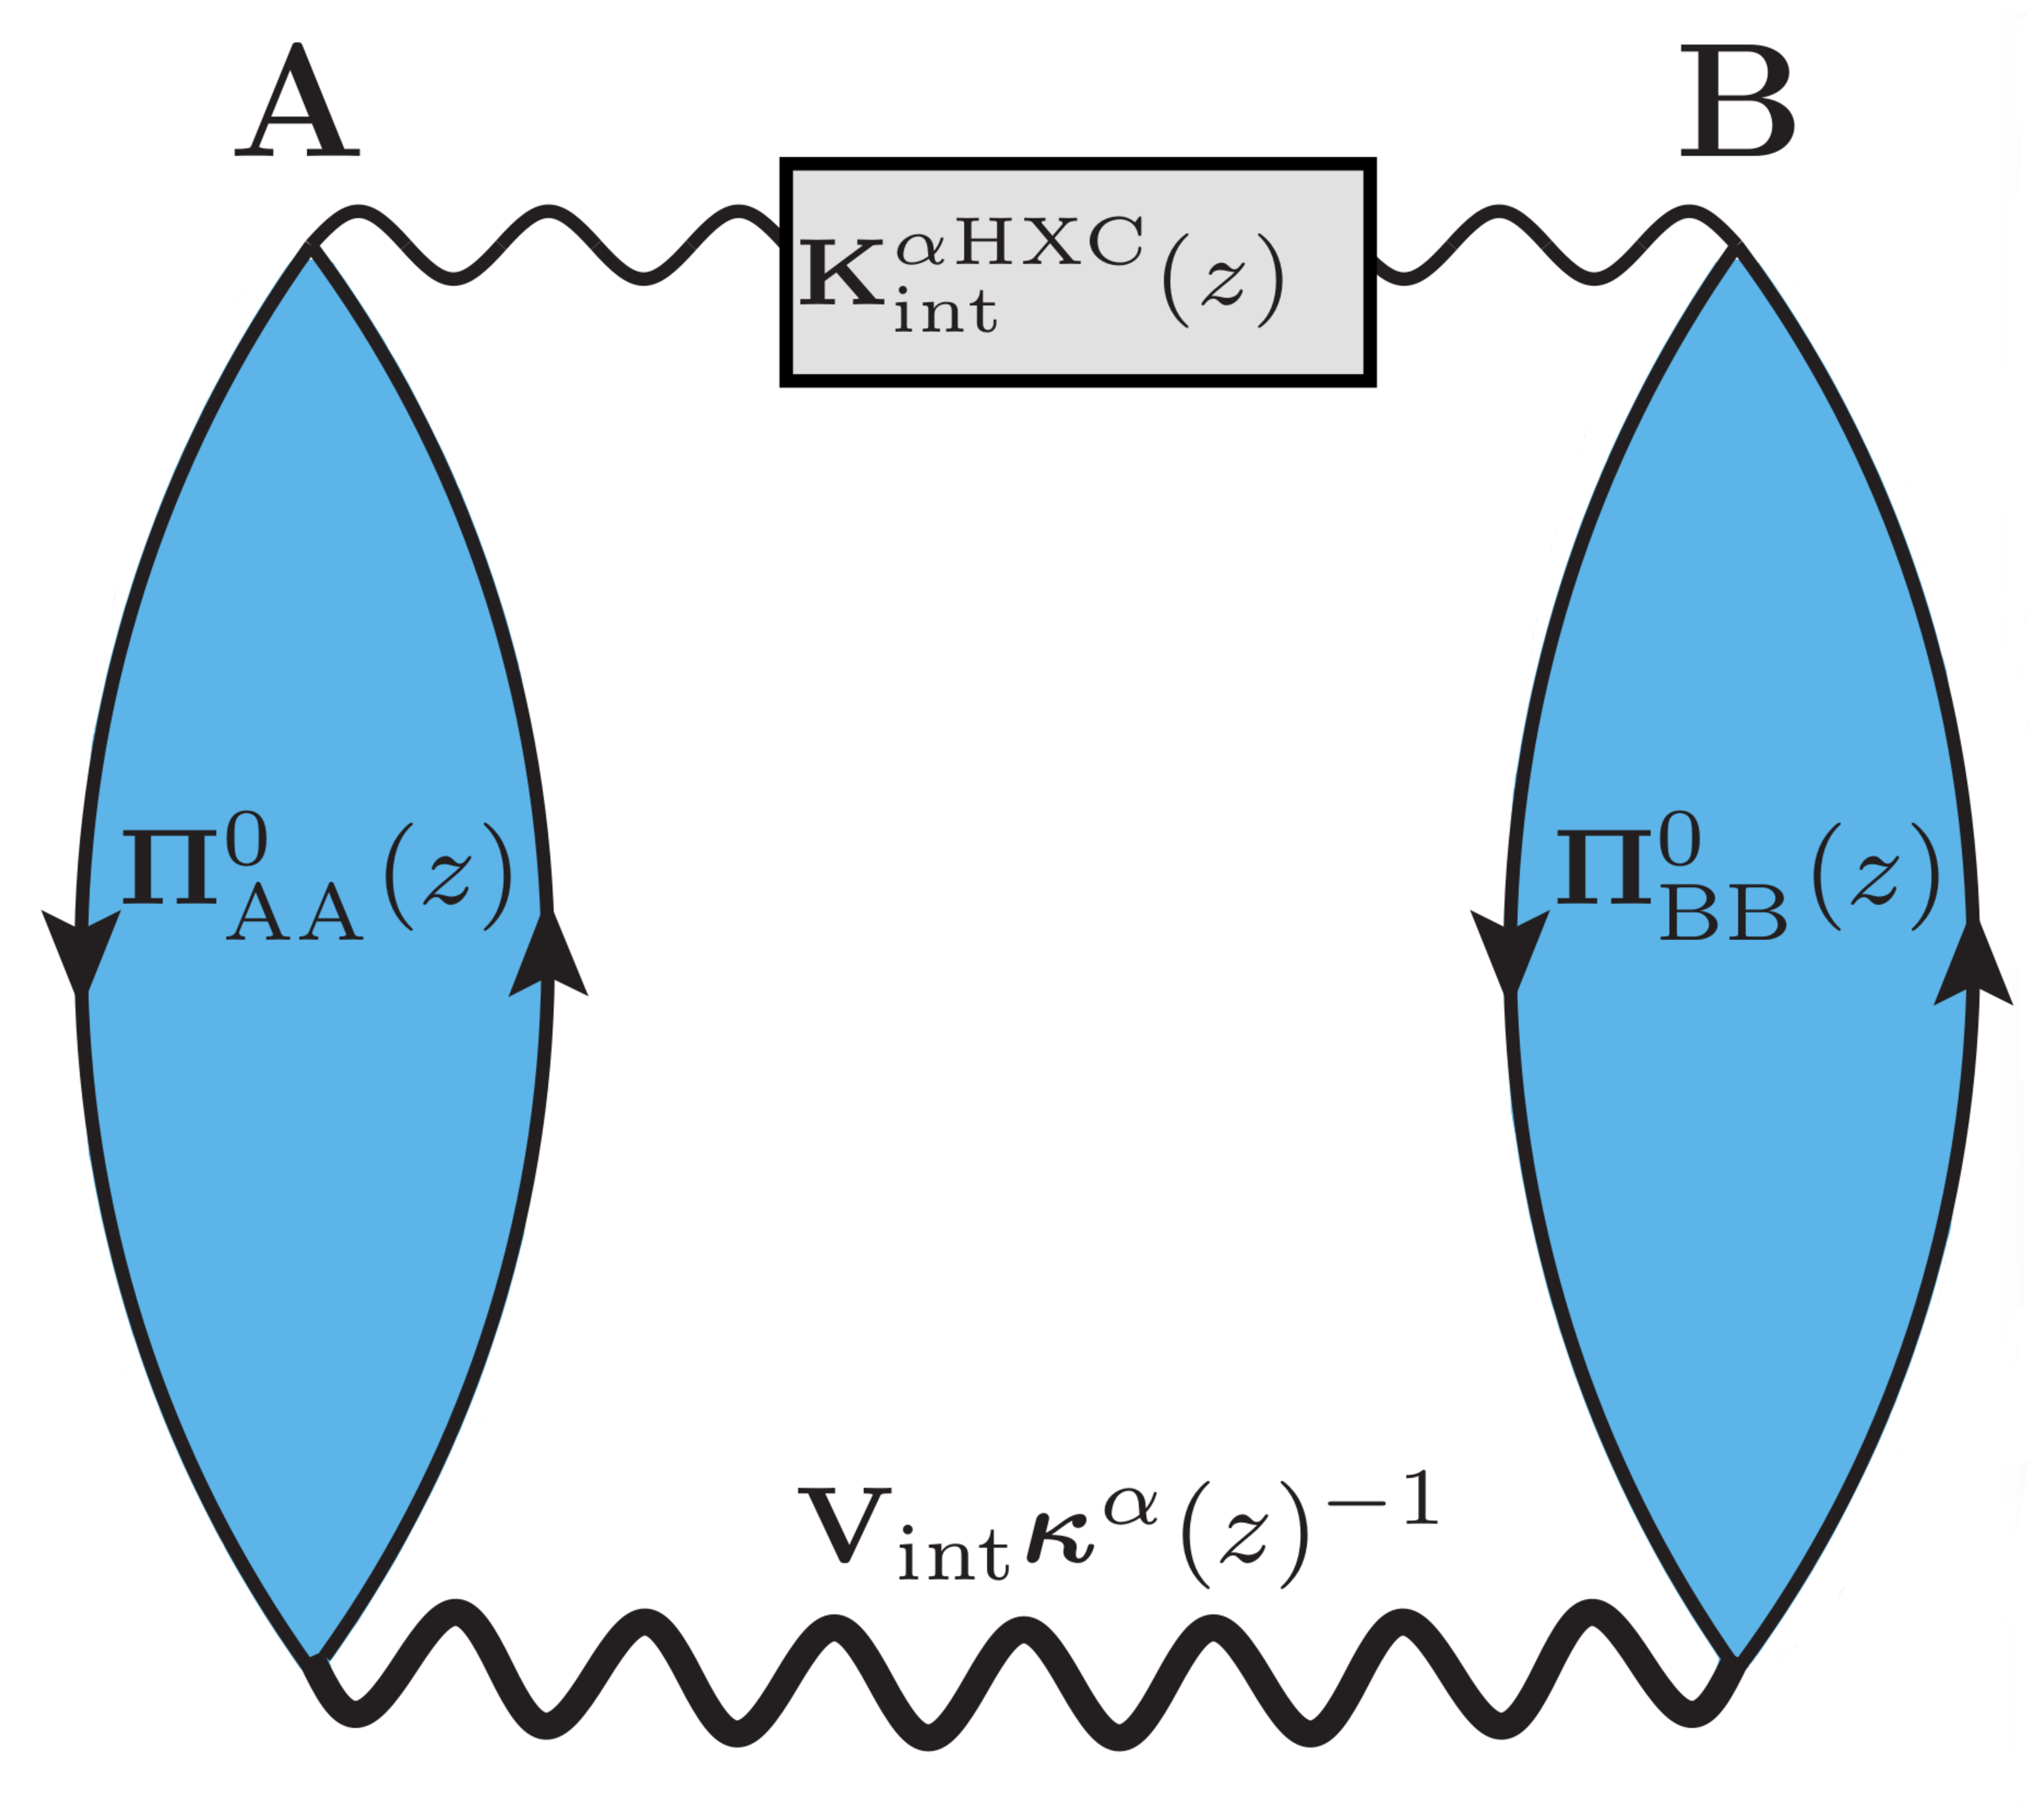
\includegraphics[width=0.5\linewidth]{int_gold.eps}
  \caption{Diagrammatic representation of the A--B dispersion energy
    Eq. (21). \rev{Blue-shaded} rings with upward--downward
    arrows denote particle--hole propagators of the monomers containing
    the full intra-monomer interaction, whereas horizontal \rev{wavy} lines
    represent interactions between the monomers. Coupling strength and
    frequency integration \rev{are} implied.}
  \label{fig:goldstone}
\end{figure}

\begin{table}[H]
  \caption{Parameters of the \rev{\sout{the}} linear regression
    fits displayed in Figure \rev{10}. The slope corresponds to the 
    average relative interaction energy error \rev{($\%$)} per valence
    electron (VE), and the $y$-intercept corresponds to the average
    relative interaction energy error \rev{($\%$)} in the limit of zero VEs.} 
  \begin{tabular}{lRR}
    \hline
    \text{Method} & \text{Slope (\%/VE)} & y\text{-intercept (\%)} \\
    \hline
    \text{MP2} & 0.1219 & 7.30 \\
    \text{SCS-MP2} & 0.0251 & 14.10 \\
    \text{RPA(PBE)}& 0.0030 & 6.24 \\
    \text{PBE-D3}  & 0.0083 & 6.79 \\
    \hline
  \end{tabular}
  \label{tab:slopes}
\end{table}

\begin{figure}[H]
   \centering
  \includegraphics{deviate_v4.eps}
  \caption{Errors in ROT34 computed rotational constants compared to
    experiment.\cite{Risthaus14JComputChem35p1509}  
    Mean absolute errors (MAE) and mean errors (ME) are in MHz,
    and relative minimum-maximum error ranges
    (rMinMax) are in $\%$. MP2 and SCS-MP2 results are from
    Ref. \citenum{Risthaus14JComputChem35p1509}; and SCAN, SCAN-D3,
    \rev{PBE-D3}, and M06L results are from Ref. \citenum{BrandenburgPhysRevB}.}
  \label{fig:methods_bar}
\end{figure}

``As a result, \rev{unscreened} perturbation theories produce exaggerated
responses of the monomers to external perturbation \rev{and} divergent estimates
for NIs even in moderately large systems.'' (p. 33)

3) The choice of basis set for the halogen bond complexes from
the S30L was added to Section 2.2 on p. 7:

``RPA correlation energies were evaluated using Dunning's correlation-consistent
  polarized valence basis sets\cite{Dunning89JChemPhys90p1007,doi:10.1063/1.464303}
  in conjunction with the corresponding auxiliary correlation-consistent basis
  sets optimized for RI-MP2.\cite{Weigend02JChemPhys116p3175,b415208e}
  \rev{Small core relativistic effective core
    potentials\cite{doi:10.1063/1.1622924,doi:10.1021/jp065887l} were used for
    the halogen atoms in the S30L\cite{Sure15JChemTheoryComput} benchmark set.}''
    (p. 7)

4) The section title was updated:

``\textbf{4.5 Approximations \rev{within AC-SAPT}}'' (p. 21)

5) We added a sentence in the conclusion to emphasize
  the lack of empirical parameters in our approach:

``Our conclusions regarding the divergence of MBPT for NIs
  rely in part on the assumption that the RPA dispersion energy is
  qualitatively accurate, which is supported by the close agreement
  between the RPA and the benchmark results. \rev{This agreement is
    remarkable given that RPA is parameter-free aside from using
    a KS reference from a semilocal DFA.}'' (p. 35)

6) We modified the supporting information to clarify the choice of basis sets for the halogen
  bond complexes of the S30L\cite{Sure15JChemTheoryComput} test set with footnotes at the bottom of
  Tables S6, S7, and S8:

\rev{\textsuperscript{\emph{a}} Halogen
    atoms used correlation consistent small core relativistic
    pseudopotentials.\cite{doi:10.1063/1.1622924,doi:10.1021/jp065887l}}

%%%%%%%%%%%%%%%%%%%%%%%%%%%%%%%%%%%%%%%%%%%%%%%%%%%%%%%%%%%%%%%%%%%%%
%% The appropriate \bibliography command should be placed here.
%% Notice that the class file automatically sets \bibliographystyle
%% and also names the section correctly.
%%%%%%%%%%%%%%%%%%%%%%%%%%%%%%%%%%%%%%%%%%%%%%%%%%%%%%%%%%%%%%%%%%%%%
\bibliography{references}

\end{document}
